\label{sec:protodune}
\subsection{The Prototypes}
The \pd program will help validate various DUNE technology aspects before proceeding with the construction of the principal DUNE detectors at SURF.
It is designed for measurements with a test beam provided by a dedicated target and beamline system at the CERN SPS accelerator complex.
It also has the potential to be an important platform for realistic Liquid Argon Time Projection Chamber (LArTPC) detector characterization
(e.g. PID, shower response, etc.) utilizing controlled conditions of a test-beam experimental setup. The name ``\pd'' currently applies to two
full-scale LArTPC prototypes based on two different technologies --- single-phase (SP) and dual-phase (DP) TPCs.
The ``full-scale'' designation is used to describe the fact that the prototypes
contain important (and large) structural and readout elements built according to the specifications
of the eventual full detector (including the size).

The ``single-phase''  LArTPC functions without amplification in the medium (liquid Argon) and is in essence a very large ionization chamber
equipped with a large number of readout electrodes (wires), each with its own electronics chain. In this design, the front-end electronics is
situated within the cryostat in order to minimize noise (the so-called ``cold electronics design'').

In the ``dual-phase''  TPC ionization
electrons are extracted from the liquid into the gaseous phase of Argon, and drift in Argon gas towards a specially designed 2D structure
on top of the detector where they multiply according to principles of proportional chamber operation. The two designs are complementary
in the sense they explore different technologie and approaches to optimization of the Liquid Argon detector characteristics.

Both  proposals have been approved and the dual-phase prototype was given the official designation as a CERN experiment \textbf{NP02},
while the single-phase was designated as \textbf{NP04}. They will be built and deployed at CERN in 2017 and scheduled to take data in 2018.
The prototypes will be placed in a specially constructed large-scale extension of the existing experimental hall located in the CERN North Area.
Each prototype will be provided a dedicated optical fiber network connection to the CERN central storage facilities located in the West Area
campus of CERN. The nominal bandwidth of these dedicated network connections will be 20\,Gbps for each experiment.
% The motivations for this specific choice of nominal bandwidth will be presented in the following sections.

% ----------------------------------------------------------
\subsection{\pd Glossary}
\begin{description}
\item{CASTOR} archival tape storage at CERN
\item{Enstore} archival tape storage at FNAL
\item{EOS}  high-performance distributed disk storage system at CERN
\item{F-FTS} Fermilab File Transfer Service
\item{NP02} The dual-phase part of the \pd program
\item{NP04} The single-phase part of the \pd program
\item{QA} Quality Assurance (mostly applied to the recorded data in this context)
\item{RDMS} Raw Data Management System
\item{SAM} Metadata and File Catalog at FNAL, interfacing mass storage
\end{description}


\subsection{The protoDUNE Data Characteristics}

In order to provide the necessary precision for reconstruction of the ionization patterns in the LArTPC, both single-phase and dual-phase designs share the same fundamental characteristics:
\begin{itemize}
\item High spatial granularity of readout (e.g. the dense electrode pattern), and the resulting high channel count
\item High digitization frequency (which is essential to ensure a precise position measurement along the drift direction)
\end{itemize}

\noindent
Another common factor in both designs is the relatively slow drift velocity of electrons in Liquid Argon, which is of the order of millimeters per microsecond,
depending on the drift volume voltage and other parameters. This leads to a substantial readout window (of the order of milliseconds) required to collect
all of the ionization in the Liquid Argon volume due the event of interest. Even though the readout times are substantially different in the two designs,
the net effect is similar. The high digitization frequency in every channel (as explained above) leads to a considerable amount of data per event.
 Each event is comparable in size to a high-resolution digital photograph.

There are a few data reduction (compression) techniques that may be applicable to \pd raw data in order to reduce its size. Some of the algorithms
are inherently lossy, such as the so-called \textit{Zero Suppression} algorithm which rejects parts of the digitized waveforms in LArTPC channels according
to certain logic (e.g. when the signal is consistently below a predefined threshold for a period of time). There are also lossless compression
techniques such as Huffman algorithm and others.

\textbf{At the time of writing it is assumed that only the lossless algorithms will be applied during the compression
of the \pd raw data, while zero suppression is considered a separate option that may be implemented when taking a portion of the data.}

It is foreseen that the total amount of data to be produced by the \pd detectors will be of the order of a few
petabytes (including commissioning runs with cosmic rays). Instantaneous and average data rates in the data transmission chain are expected to be
substantial (see \ref{sec:np02_online_processing} and \ref{sec:np04_data_rate}).
For these reasons, capturing data streams generated by the protoDUNE DAQ systems, buffering of the data, performing fast QA analysis,
and transporting the data to sites external to CERN for processing (e.g. FNAL, BNL, etc.) requires significant resources and adequate planning.

\subsection{Raw Data Flow in \pd: the Concept}
\label{sec:raw_concept}
%%%%%%%%%%%%%%%%%%%%%%%%
\begin{figure}[tbh]
\centering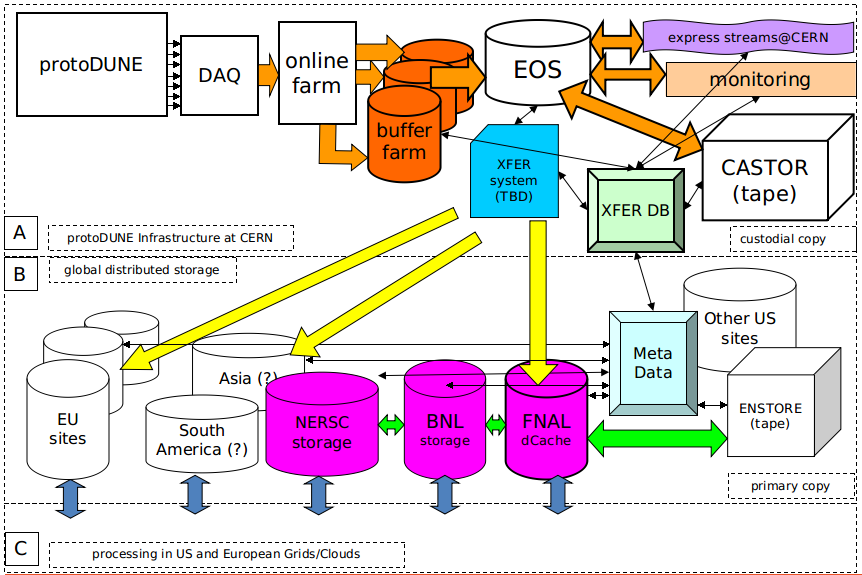
\includegraphics[width=\linewidth]{protoDUNE_raw_data_concept.png}
\caption{\label{fig:raw_concept}Conceptual diagram of the flow of raw data in \pd}
\end{figure}
%%%%%%%%%%%%%%%%%%%%%%%%

\noindent
Conceptual diagram of the raw data flow in \pd is presented in Fig.\ref{fig:raw_concept}. It shows the general logic
of data flow, and does not include specific assumptions about what system will be used to actually move the data.
It also reflects the central role of EOS in the \pd raw data management scheme. This is motivated by the experience
and architecture of the LHC experiments. EOS serves as the staging area from which the data gets committed to CASTOR
and from which it is transmitted to a number of endpoints including principal data centers such as FNAL and others.
It is also used to provide input to QA and other express processing streams at CERN (which fall into the ``prompt use'' category).
This scheme assumes that there is no conceptual difference between NP02 and NP04 in terms of the general pattern of data flow.

Data centers at BNL and NERSC are placed in this diagram for illustration purposes. Any other institution possessing adequate
resources can participate in this data distriburtion scheme if desired.


\subsection{Prioritization}

All of the many elements in the chain of data acquisition, storage, distribution and processing are critically important to derive physics results  from the data.
At the same time, certain components of the data chain need to be prioritized over others in order to reliably perform the measurements during a potentially
limited time period (depending on the SPS and LHC running schedule).

The priority components are the DAQ and the Raw Data Management System (RDMS), which includes capturing the data coming out of the DAQ,
transporting the data to persistent mass storage and prompt Quality Assurance which is required to ensure corrective action can be taken
if the detector or certain system problems are identified in the QA process. In NP02, major processing including QA will take place
on a purpose-built storage and processing farm located in immediate proximity of the DAQ (see~\ref{sec:np02_online_processing}).

In NP04, data samples will be processed for QA purposes on the CERN batch facility (and perhaps at FNAL if low latency can be
achieved for data transmission). The latter can be thought of as a more sophisticated monitoring done in near-time in addition to the in
situ monitoring done with DAQ, which implies a ``few minutes'' scale of processing.


\subsection{RDMS Requirements}
\subsubsection{A Note on the File Size}
At the time of writing, the raw data file size in protoDUNE  is assumed to be \filesize (nominally). A few metrics in the data management area depend of this
parameter, for example the total number of files produced by the experiment, rate of file registration in the database etc. This can be adjusted
later as needed and is used here primarily for estimation purposes.

\subsubsection{DAQ Interface: buffering requirements}
\label{sec:daq_interface}
The plan is to have sufficient buffering capability in the DAQ for both NP02 and NP04. In this case, ``sufficient''
primarily means conforming to the CERN requirement that the experiment must be able to keep taking data for a
least 3 days at the nominal data rate, even if there is an occasional problem with the data link between the
experiment site and CERN central storage facilities, or an issue with the central storage systems or any type of similar outage.
On top of that, NP02 has substantial additional requirements as explained below:
\begin{description}

\item[NP02] The planned buffer depth is rather large (petabyte scale), in order to enable a substantial amount of
processing locally at the site of the experiment, in accordance with the existing plans (see~\ref{sec:np02_online_processing}).
 To make this possible the design calls
for deployment of the necessary computing resources (equivalent to hundreds of cores) in the data room of NP02. A number of options are being explored
for the NP02  storage solution, including GPFS and XRootD.
%Clearly this goes beyond the concept and functionality of a simple buffer as
%it also needs to perform as a high-throughput staging area for local processing.

\item[ NP04] In the single-phase experiment the emphasis is on a more lightweight and fault tolerant setup which satisfies the general buffering and throughput requirements.
No extensive processing is foreseen on the experiment site. Among the possible technical options for the buffer farm file access is XRootD.
\end{description}

\noindent
It is this outer layer of the data acquisition system (the buffer) in each experiment that will need to be interfaced with
the rest of the \pd raw data management complex.  It is represented as the block labeled ``buffer farm'' in Fig.\ref{fig:raw_concept}.

In summary, NP02 and NP04 will use the ``buffer'' in two very different ways.  In NP02
the storage local to the experiment will serve to host the data which will be subject to active processing at a considerable scale
and simultaneously with the data taking (i.e. effectively in real time).
It is obvious that the storage system in NP02 has functionality beyond that of a simple buffer (which is mostly the case in NP04)
and serves as an active staging area for local processing. This has a number of consequences such as the need to plan
for simulataneous read and write operations on the same storage system, taking place at a considerable rate.

\subsubsection{Functional Requirements for Data Management}
\label{sec:func_reqs}
The following is a summary of basic requirements for the \pd data management system:
\begin{itemize}

\item Transfer raw data files from both NP02 and NP04 online disk buffer farms
to CERN EOS disk and from there to CERN tape (CASTOR), FNAL tape (Enstore) and other end-points.

\item Ensure that the throughput is adequate and there are no bottlenecks for the Data Acquisition System
given the expected data rates

\item Record file metadata inculding the file status and outcome of file operations

\item Operate at CERN and FNAL with support for initial setup and ongoing operations

\item Provide monitoring of overall system health, detection of error conditions and corresponding alerts, and support of troubleshooting

\item As a part of functionality described in the previous item, perform checksum comparison for each leg of data transfer, for
example during data transport from the experiment to EOS and beyond

\item Provide triggers to perform file operations (copy, delete) based on configurable rules

\item Support ``express lane'' processing at CERN and other institutions

\end{itemize}



% ----------------------------------------------------------
\subsection{Outline of the NP02 online processing plans}
\label{sec:np02_online_processing}
The online processing in NP02 will be sized in order to process all beam data produced at the nominal rate of 100\,Hz. 

The idea is to disentangle $\sim$70 cosmic ray tracks overlapping each beam event in the $\pm$4ms around the beam trigger
and to exploit the light readout information in order to reconstruct the real drift coordinates of these tracks.
Then one or two tracks per event satisfying certain requirements such as track length and angle are selected for the monitoring and
data QA tasks. The idea is to use them first for purity assessment and once the purity is determined to measure the gain in all
channels. By accumulating information from many events the system can provide an online monitoring of the status of the detector
and data quality. Also subject to monitoring will be some event parameters which are representative of the different kind of events and
beam energies.
% in order to check that the samples do not change with time during data taking.

In the above the following assumptions are made which are based on a few known features of dual phase:
\begin{itemize}
\item easy reconstruction due to only two collection views and high signal-to-noise
\item reasonable number of readout channels (7680)
\item use of existing QSCAN software for fast reconstruction
\item data compression factor of at least 10
\end{itemize}

\noindent This kind of online data treatment is  different with respect to what one would perform
more generally offline. The use of the CERN batch system for this online analysis is not foreseen.

In general, the data produced by the online processing system will not be saved to mass storage for presevation, with
the exception of small subsets for purpose such as the online event display and others. Statistical information will be gathered by
the monitoring software and saved from time to time.

Design of the data and workflow management required to make possible processing strategy outlined above is work in progress
at the time of writing.

% ----------------------------------------------------------
\subsection{Estimates of the NP04 data rates}
\label{sec:np04_data_rate}
The buffer farm in the single-phase experiment NP04 serves to satisfy
the CERN IT requirements for experiment-local storage and also as a necessary
staging area from which the data can be committed to CERN EOS without impacting the operation
of the DAQ and other online systems. Parameters of the farm and the NP04 computing model
as a whole will be driven by the data volume and rate. At the time of writing, understanding of the data
characteristics is incomplete and a range of possibilities must be considered. The leading
possibilities are documented in the spreadsheet in DUNE DocDB 1086\,\cite{duneDocDb1086}.
One of the most likely scenarios is summarized in Table~\ref{tab:np04_data_rate}. The size of
the buffer includes a provision based on the working assumption that a cosmic muon trigger will
be taken for each beam event trigger, in order to perform various calibrations.

\begin{table}[htbp]
  \centering
  \begin{tabular}[h]{l|r}
\hline
    Trigger rate & 25\,Hz \\
    Spill duration & 4.5\,s\\
    SPS Cycle & 22.5\,s \\
    Readout time window & 5\,ms \\
    \# of APAs to be read out & 6 \\
    \hline
    Single readout size (per trigger) & 230.4\,MB \\
    Lossless compression factor & 4 \\
    Instantaneous data rate (in-spill) & 1440\,MB/s \\
    Average data rate & 576\,MB/s \\
    \hline
    3-Day buffer depth & 300\,TB \\
    \hline
  \end{tabular}
  \caption{Parameters defining data rate and volume in the ``central'' scenario v5\,\cite{data_spreadsheet}, including both
  the in-spill and out-of-spill data.}
  \label{tab:np04_data_rate}
\end{table}

\noindent It's worth mentioning that under any scenario it will be necessary to perform writing to disks in parallel
to have adequate bandwidth; every disk will have simultaneous write and read operations performed on it, since
it's a buffer and not the final destination of the data.



\subsection{ The Raw Data Characteristics}
\subsubsection{NP02}
Outline of the online processing plans for NP02 is presented in Sec.\,\ref{sec:np02_online_processing}.
As follows from this description, and in constrast to NP04, data will not be streaming to mass storage at
the same average rate as it is produced in the detector systems, and instead recorded selections of data
will be transferred to EOS and external sites from time to time in a managed manner, based on operators' decision.
The pattern of this transfer is not yet defined. Nominal total volume of data to be preserved is 2.5\,PB.

%Data volume and rate for NP04 is presented in Sec.\,\ref{sec:np04_data_rate} for three
%different scenarios.
%The ``medium rate'' scenario is characterzied by an instantaneous rate of 0.23\,GB/s and
%average rate of 0.07\,GB/s, with total data volume of 0.23\,PB. However, for planning
%purposes it is helpful to consider the maximum rate and volume scenario in order to better
%understand the limits of  scalability of
%the system in case such scenario will be realized. According to Table\,\ref{tab:np04_data_rate}
%th total amount of data for the extreme case in NP04 is 1.2\,PB. This information
%is summarized in Table~\ref{fig:det_perf}.
%\begin{table}[tbh]
%\centering
%\begin{tabular}{l l l}
%\hline
%\textbf{Performance Benchmark} & \textbf{Single Phase} & \textbf{Dual Phase}\\
%\hline
%\hline
%Raw data volume (total, PB)                    & 1.2\,PB & 2.5\,PB \\
%Raw data files (total, thousands)            & 240  & 500\\
%Average Rate to Mass Storage & 3.3\,GB/s & N/A \\
%Avg. Data Rate                                & 20\,Gbps & 20\,Gbps \\
%Latency to reach EOS                     & 10\,min & 10\,min\\
%Latency to reach express lane processing & 10\,min & 10\,min\\
%\hline
%\end{tabular}
%\caption{\label{fig:det_perf}Expected protoDUNE data characteristics.}
%\end{table}

\subsubsection{NP04}
At the time of writing, the nominal number of triggers to be recorded in NP04 is 25\,M.
Combined with the readout size quoted in Table\,\ref{tab:np04_data_rate}, this leads to
the estimate of 5.7\,PB for the total data volume for beam events..

Each of NP02 and NP04 experiments will be provided with a network connection of 20\,Gbps
bandwith, which effectively defines the upper limit on the average data rate
produced in each experiment.


% The file handling system assumes the following limits will not be exceeded (Table~\ref{fig:dh_perf})
%\begin{table}[tbh]
%\centering
%\begin{tabular}{l l l}
%\hline
%\textbf{Performance Benchmark} & \textbf{Single Phase} & \textbf{Dual Phase}\\
%\hline
%\hline
%Pending files in FTS dropbox             & 1~PB        & \\
%Simultaneous active files in transfer    & 50,000      & \\
%File registrations rate                  & 3600/hr     & \\
%File registrations                       & 200,000/day & \\
%\hline
%\end{tabular}
%\caption{\label{fig:dh_perf}Performance requirements for the data handling system used in the \pd experiment.}
%\end{table}

\subsection{Outline of the RDMS Design}


\subsubsection{The Fermilab File Transfer System}
The design presented here leverages the technology of the Fermilab
File Transfer System (F-FTS or just FTS), which has been successfully
applied in a number of Intensity Frontier Experiments and demonstrated
a high degree of robustness along with automation, integrated metadata
and extensive monitoring capabilities.

Fig.~\ref{fig:ftsbasics} shows a cartoon of the basic functionality
of a single FTS instance.  A FTS instance is bound to one or more
sources of input or ``dropboxes'', which it  periodically polls.
As new files are discovered the FTS instance will initiate transfer of the file to its endpoints.
Transfers may be handled directly by FTS or may be delegated to one of
several $3^\mathrm{rd}$ party mechanisms, as schematically illustrated
in  Fig. \ref{fig:ftsbasicsthird}.

A dropbox may be a POSIX-like file system directory or a source of data accessed
through a network protocol layer (such as  XRootD, gridFTP etc). The frequency at
which the dropbox is polled is configurable and will be a component of the overall latency
of the data transfer.

The lifetime of a file in a dropbox is under the control of the FTS
instance.  A file must appear in a dropbox in an atomic manner
(e.g. via the \texttt{mv} command). In all other respects the producer
of a file runs independently from any FTS instance.  Depending on the
nature of the dropbox, multiple file producers may provide input files.


As described in section~\ref{sec:cleanup}, the file is eventually removed from the
dropbox by the FTS.  Depending on the rules for cleanup, an opportunity
exists for ad-hoc or other ``prompt processing'' of the data files while
they reside in a dropbox. Fig.~\ref{fig:ftsbasics} includes a reference to the possible
``prompt processing'' which for example may be required to enable
near-time monitoring. Finally, throughout these actions (discovery, transfer,
removal), a record of the state of the file is maintained in a SAM
database (section~\ref{sec:sam}).

\begin{figure}[tbh]
  \centering
  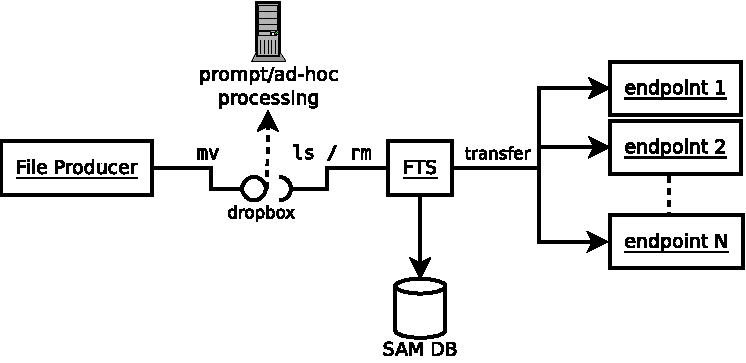
\includegraphics[width=0.8\textwidth]{fts-basics.pdf}
  \caption{Basic functionality of an FTS instance with a single input dropbox.
Prompt processing of the data while it resides in the dropbox depicted in this diagram is optional.}
  \label{fig:ftsbasics}
\end{figure}

\begin{figure}[tbh]
  \centering
  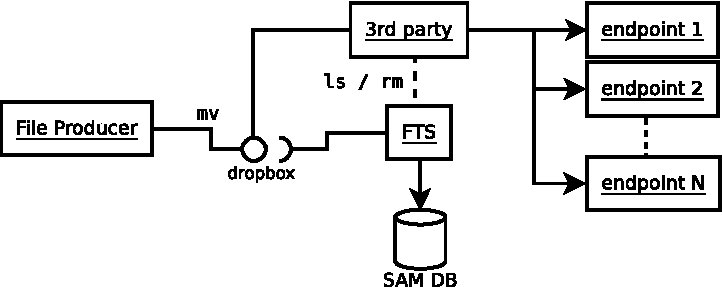
\includegraphics[width=0.8\textwidth]{fts-basics-3rd.pdf}
  \caption{Basic functionality of an FTS instance which is capable of initiating third-party transfers.}
  \label{fig:ftsbasicsthird}
\end{figure}

\noindent As mentioned in \ref{sec:daq_interface} and\,\ref{sec:np02_online_processing},
NP02 has requirements for the experiment-local storage that go beyond
that of a buffer. For that reason, there will be some differences between
NP02 and NP04 in terms of placement and function of a few system components,
while others will be shared.

\subsubsection{FTS instances in NP04}
\label{sec:prim_sec}
Two FTS instances will be used to marshal raw data from the single-phase protoDUNE (NP04)
detectors in a manner presented in Fig.~\ref{fig:ftsinstances}.  The
``primary'' instance (labeled FTS-1) is responsible for transferring data
from the disk buffer farms to CERN's EOS (central distributed disk storage).
 The ``secondary'' instance (FTS-2) is responsible for transferring files from EOS to
CASTOR (tape), and also to FNAL and other recepients of the raw data set.

This tiered approach is similar to the data flow pattern in the LHC experiments and achieves several goals,
as outlined in Sec.\,\ref{sec:raw_concept}. In particular
it makes possible prompt use of the files residing in EOS, as explained below.

\begin{figure}[tbh]
  \centering
  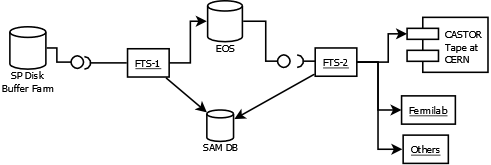
\includegraphics[width=0.7\textwidth]{ftsinstances_v2.png}
  \caption{The two instances of FTS used for marshaling raw data from the protoDUNE detectors.}
  \label{fig:ftsinstances}
\end{figure}

\subsubsection{FTS instances in NP02}
NP02 will also rely on FTS to transfer data from EOS to tape and remote sites such as FNAL,
so the block ``FTS-2'' in the diagram presented in the diagram in Fig.~\ref{fig:ftsinstances} will still be in place.
However, the system to move the data from the experiment-local storage to EOS will be specified at a later date,
and be subject to the requirement that there is minumum interference between the real-time processing
taking place on site and data transfer to EOS.

\subsubsection{Express Streams and other ``Prompt Use''}
\label{sec:prompt}

While raw data files are available on EOS they can be
used for a number of purposes, such as express streams and
other prompt processing for monitoring and QA purposes,
and also as a data source for production taking place at CERN, which is under preliminary
consideration. Specifics of the latter have not been  worked out at the time of writing
and will be one of the work areas prior to \pd commissioning.
An example of data flow is shown in Fig.~\ref{fig:prompt}.

\begin{figure}[tbh]
  \centering
  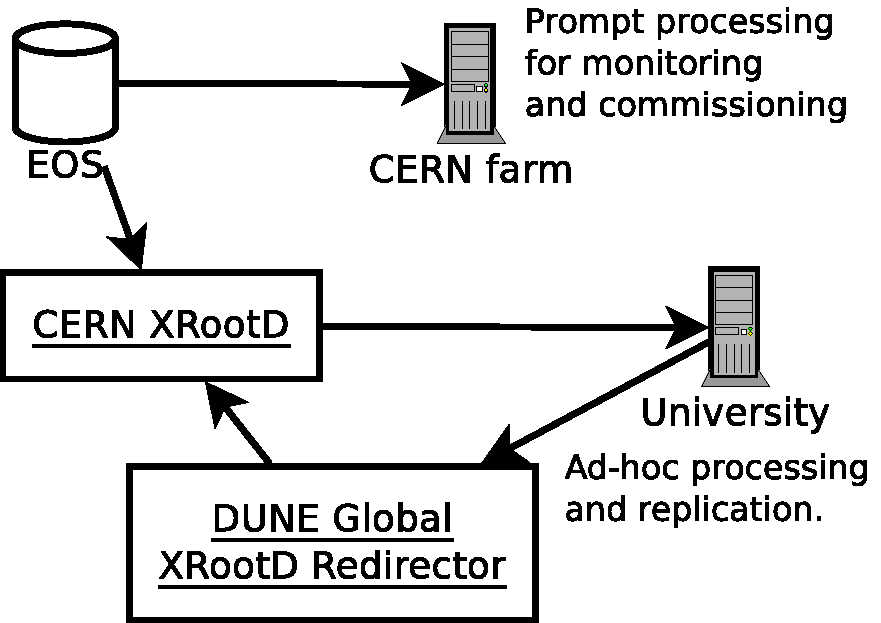
\includegraphics[width=0.5\textwidth]{prompt.pdf}
  \caption{Scenarios for prompt access and processing of raw data files.}
  \label{fig:prompt}
\end{figure}

%Prompt processing will be performed at CERN on a subset of the raw
%data to support commissioning and ongoing data quality monitoring.

\noindent Collaborators at universities or other institutions will have ad-hoc
access to the files while they are on CERN EOS via XRootD and other mechanisms if desired. 
The data catalog (Sec.~\ref{sec:sam}) will be used to identify global file
locations which will be resolved through the DUNE XRootD redirector or
through cache layers such as the ``Stash Cache'' system employed by
the Open Science Grid.

\subsubsection{Data Catalog}
\label{sec:sam}

Underlying FTS will be a fully featured data management layer
implemented with Fermilab's \textit{Serial Access to Metadata} (SAM) system.
It will provide file metadata, fileset definitions and replica
catalogs.  All data being handled by the transfer systems will have
corresponding records in the data handling catalog so that the
content, locations and provenance of the data can be fully tracked.
The primary catalog systems will reside at FNAL with proxy/cache
layers in Europe and North America (see \ref{sec:replication}
for more details on data replication) to ensure high speed,
low latency connections between the servers and the (offline analysis)
clients that will query the catalogs from these zones.  Similar
scalable proxy and cache layers can be instantiated in other regions as required.

\subsubsection{Deletion and Cleanup}
\label{sec:cleanup}

An FTS instance handles the ``cleanup'' of its input dropbox, with
configurable, periodic cleanup passes through its current file sets.
An example cleanup process is shown in flow chart of
Fig.\ref{fig:ftscleanup}.  Central to this is a configurable
multi-stage validation procedure to determine if files are eligible
for deletion/cleanup from the input area.  In particular, cleanup
performed by FTS-1 can be based on the successful archive of the file
to CASTOR performed by FTS-2 through metadata recorded in SAM.

The system may also provide an ``age'' criterion on files so that
files can be retained for time periods that are longer than required
just to reach their ultimate FTS endpoints.  This allows time for
operations like online/nearline processing of files remaining in the
dropbox or to allow investigation of recent log files.


\begin{figure}[tbh]
  \centering
  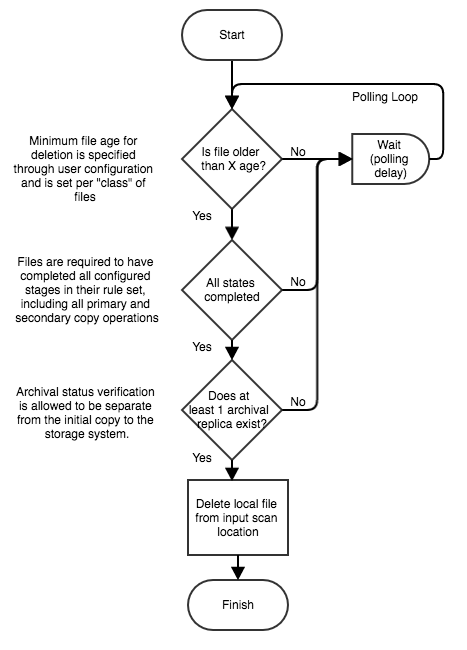
\includegraphics[width=0.55\linewidth]{fts_file_deletion_flowchart.png}  
  \caption{Flowchart of the \pd file deletion and cleanup.}
  \label{fig:ftscleanup}
\end{figure}


 
\subsection{Technical Requirements to the FTS Components}

\subsubsection{Outage and Backlog Considerations}
\label{sec:backlog}
As already mentioned in Sec.\ref{sec:daq_interface},
CERN policies require that an experiment is capable of storing data locally (in the vicinity of the apparatus as opposed to CERN Central
Storage)  for a nominal period of 3 days, to ensure that the experiment can run for a period of time even in case of network interruptions
and storage facility outages.

In an outage scenario the data preserved locally must still be committed to mass storage when services are
restored after an outage. This creates a backlog situation which roughly doubles the requirements on the sustained
rate of file registration and other transactions, buffer areas and certain other parameters of the overall system.
This will be reflected in some of the estimates presented below.


\subsubsection{Data Throughput}

The data management system must perform in a way that allows to fully leverage the underlying hardware and networking infrastructure
upon which  it is running.  In the case of the \pd experiments the FTS system will be capable of operating at a sustained data processing and transfer
rate that is greater than 80\% of the maximum theoretical bandwidth available between the DAQ buffer farms and the EOS storage system.
In the current design this network bandwidth consists of two 20\,Gb/s ethernet links (one for each experiment).
%  The RAID arrays or distributed file system architectures to which the data will be written to and read from are assumed
% to have similar or lower available bandwidth.
This sets the upper limit of the throughput of the entire system, with other components operating at this or perhaps lower levels.
The actual observed read/write bandwidth will be determined by configuration of the detectors and the combination
of the DAQ hardware and software.


  The primary DAQ FTS system will be required to operate at a sustained effective bandwidth
of the lesser of: two times 16\,Gb/s (80\% of theoretical network bandwidth) or 80\% of the measured read access bandwidth from the storage arrays
of the buffer farms
(during simultaneous write operations, if the DAQ computing models requires this mixed access mode) under the standard \pd operations.

\subsubsection{Transaction Throughput}

In terms of transaction handling,  the data management system must be capable of efficiently using the data
catalog and infrastructure in order to meet or exceed the rate at which files or other data
objects are generated by the \pd detectors amd their DAQ components.

For NP04, where the data are captured in files and transmitted continuously to mass storage while
the experiment is running, the following considerations are applicable to the transaction rate.
Given the nominal file size of \filesize (nominal, used here for estimation purposes), 
the primary FTS system must be able to support a minimum transaction rate of up to  $\sim$1\,s$^{-1}$
and the corresponding aggregated total of $\sim$10$^5$ file registration operations per day.
This level of performance has been demonstrated in other deployments of this type of data
handling system.

In case of NP02, the data are not written to files continuously and rather there will be periods when
select data samples are captured, registered in the file catalog and shipped out to mass storage.
Since this use case is still subject to the nominal cap of 20\,Gbps bandwidth of the network connection
to the CERN central services, the order of magnitude estimates are same as for NP02 in terms of transaction rate.

\subsubsection{Transaction Tracking}
The data management system must be able to perform simultaneous end-to-end tracking
of all files that are in state of transit the system prior to being written/verified in the archival storage,
without impacting or interrupting data taking. 

To achieve this goal the transaction tracking system for \pd will be
able to support a total number of ``in flight'' files per FTS instance equal to the nominal number of daily transactions
(estimated above as $\sim$10$^5$) times the maximum supported duration (in days)
of an outage in the downstream network or storage domain, that can be sustained by the DAQ system.
As mentioned above, such duration is defined as 3 days per the CERN policies. In addition, due to data backlog considerations
(see \ref{sec:backlog}) there must be another factor of 2 added to guarantee transport of all data to its destination during
the recovery period. As a result, the FTS systems must support at least 6$\times$10$^5$ files in state of transit at any given time,
where at least 10$^4$ of these files are undergoing ``active'' registration/transport through the system at any given time.
In other words, $\sim$10\,k of the files are being actively
managed and their status is constantly updated while the remainder are ``waiting'' in the designated dropbox location.

\subsubsection{Transfer Latency}
The file transfer and management systems are designed to operate asynchronously with other components of the \pd DAQ
and other online systems.
Due to the polling models employed in this asynchronous model, many operations do not have fixed temporal relations to other events in the DAQ,
but rather will take place and complete within a well defined time window or with a certain latency.  In the case of the \pd experiment,
the data management systems will be capable of operating as detailed below.

In FTS-1 (see\,\ref{sec:prim_sec}), the latency between the completion of the DAQ writing a file and the hand-off/detection of the file by the
system will be controlled by a configurable delay parameter (in minutes) which defines the polling intervals for the FTS
to look for  incoming files in its input dropbox locations.  Under normal (steady state) operation, the average latency will be 1-2 polling intervals.
The actual latency may be bigger depending on the number of other new or pending files currently in the system.
In this case the order of file handling will be managed by an internal queuing algorithm that efficiently operates on the files but
does provide any user specified prioritization.

In the second stage of file transfers (FTS-2, see\,\ref{sec:prim_sec}), the time lag between the points when a file is generated by the DAQ
and when it is transferred to the EOS
system and then written to archival media (via CASTOR) -- with verification --  is dependent on the first stage latencies (new file detection and file registration)
and then the details of the archival storage system and its characteristics.  In particular the ``DAQ-to-EOS-to-CASTOR'' path will constitute a set
of chained dependencies with an independent polling interval for each stage.  Under normal operating conditions that latency for the file to
be transferred to EOS and be available through the data handling system is expected to be 1-2 of these polling cycles, contingent on write
congestion in the EOS storage system.   For full registration of the files in CASTOR and onto tape, the FTS/SAM systems will support latencies
in this recording of 3 hours to 30 days and will support a configurable timeout parameter to indicate failures in this transition.

The latency between when files are written by the DAQ and when the files are available on storage in the North American zone,
will be determined by the second stage latency of the files appearing on the EOS system from the DAQ and then a secondary latency
will be incurred based on the polling for files that require transatlantic endpoints.  Similar to the other stages this is configurable
through a polling interval.  Once queued for handling the actual file transport will be off loaded to the WLCG FTS system which will
schedule the files for transmission and will properly balance and throttle the site to site traffic and will properly conform to the CERN
 computing environment.  Latencies at this stage are well understood based on the experience that the LHC experiments have with WLCG FTS.  

\subsection{Data Management System Interfaces}
\subsubsection{Overview}
The modular design of the data handling system will provide considerable flexibility in its ability to adapt to different requirements
for interfacing  both data input and output systems.  In the \pd experiment the most important interfaces are to be established with
\begin{itemize}
\item the experiment’s core DAQ components
\item mass storage and data archival at CERN
\item mass storage and data archival at FNAL
\end{itemize}

\noindent
 Details of these interfaces are presented below.

\subsubsection{The DAQ Interface}
The interface between the core DAQ system and the data handling system is made at the DAQ’s disk buffer farm.
When the final stage event builders have completed the assembly of a file, the file will be handed off to the data handling system
by the DAQ by placing the file into a designated ``dropbox'' area on the target file system.  For POSIX compliant file systems,
this can be accomplished through an atomic move operation (i.e. Unix \textit{mv} equivalent) which minimizes the I/O overhead associated
with the hand off.  No signals need be emitted from the DAQ, nor will any other form of message be required in the direction of the
DAQ to the data handling system.  The F-FTS will detect new files through files becoming visible in configured dropbox locations of
the storage system (i.e. a new file appearing in a directory) 

The F-FTS systems running as part of the data handling system will use either a POSIX (or near POSIX) compliant file system view of the disk buffer farm,
or an API that provides access to standard meta information regarding the storage system’s dropbox area (directory) and contents
(i.e. filenames, file size, create/modify times etc…)  Additionally the FTS will require a file read API for the purpose of metadata
extraction from the file and for checksum computations (if not provided through some other means).  The system will require a
delete API and privilege, if the automated cleanup options are desired/enabled.  If the DAQ storage elements support ``third party''
transfer protocols, the FTS can use these to reduce overhead in performing the actual file transfer operations  (see Fig. \ref{fig:ftsbasicsthird}).

The organization of the FTS dropbox area(s) will be configured to support the volume of data that would be generated during a
sustained outage (of non-DAQ systems) of no less than 3 days plus the time required to register/process the volume of data
that would be generated during the outage (i.e. ``the recovery time'' required to clear a backlog).

\subsubsection{The EOS Interface}
The interface between the data handling system and the EOS storage system will be made through the APIs
provided by the standard protocols already supported by both the EOS system and the SAM data handling system.
In particular the XRootD protocol will be the primary API used for the interaction between the system, with secondary
support for the gridftp, webdav and srm protocol APIs.  The EOS system will be declared, and configured in the SAM
system as a standard storage element and will have files stored on it registered and mapped within SAM the replica
catalog to the well defined access URIs. 

\subsubsection{The CASTOR Interface}
The interface between the data handling system and the CASTOR archival storage system for file ingest will be made through the
APIs provided by the standard protocols already supported by both the CASTOR system and the SAM data handling system.
In particular these system both already support the xrootd protocol, gridftp and srm.  The CASTOR API to query the tape archive
interfaces (to determine if a file has been successfully archived to tape and which tape it is located on) will be integrated into the
SAM data handling system in a manner similar to other tape systems that SAM is already aware of (i.e. Enstore)   The CASTOR
system will be declared, and configured in the SAM system as a standard tape storage system and will have files stored on it
registered and mapped within SAM the replica catalog to the well defined access URIs along with additional tape location information
to permit optimized retrieval.  Custom modules/utilities will be developed as needed as part of the SAM data handling suite to provide
additional support for the CASTOR system in performing certain operations (i.e. bulk queries or monitoring operations).
These modules/utilities will be distributed as part of the core SAM distribution.

\subsubsection{The dCache/Enstore Interface}
The interface between the SAM data handling system and the dCache/Enstore archival storage system is already fully defined and supported.
 The interface fully supports standard access protocols including xrootd, gridftp, webdav and srm as well as the proprietary \textit{dcap} protocol
and a specialized NFS implementation that provides limited basic read access for hosts with local mounts of the dCache system.
The SAM system has modules that optimize data access based on Enstore tape location information.  This interface is in wide scale
production use across many experiments including NO$\nu$A, $\mu$BooNE, the DUNE 35t prototype, MINOS and others.

\subsubsection{The SAN/NAS Interface}
Generalized SAN and NAS systems when acting as data sources (input) will be integrated to the data handling system through their
POSIX style interface if available.  When enabled as data sinks (output) for the data handling system, a front end data server(s)
running standard access protocols in the form of xrootd or gridftp will be utilized.  These will then be mapped into SAM as standard storage locations.
  
\subsubsection{Generalized Protocol Support Interfaces}
The data handling system provides a file delivery and transfer layer which acts to provide protocol abstraction
to the end users (i.e. provides a consistent command interface) and provides a protocol bridge when performing
transfer operations between dissimilar storage systems (i.e. cross protocol transfers).  The ``Intensity Frontier
Data Handling'' tool (IFHD) for \pd will support protocol integration for:
\begin{description}
\item[XROOTD] Full support will be provided for xrootd in the Fermi-SAM data catalog, F-FTS and IFDH layers.
Currently these tools support read/write access methods.  Full support for additional xrootd features (listings,
permissions modification, etc...) is currently under development.

\item[WLCG FTS] SAM, F-FTS and IFDH will support WLCG-FTS as a 3rd party or proxy transfer mechanism.
 In this mode outbound file transfers originated from the CERN domain can offloaded to WLCG-FTS so that the
data traffic across the CERN site can be properly scheduled and balanced.  Support for this mode of operation
will be integrated into IDFH or directly into the sam\_cp layer of the F-FTS. 

\item[GridFTP] This protocol is fully supported for most of the components involved, but is not the preferred or
documented interface for any of the CERN storage components.

\item[SRM] This protocol is fully supported for most of the component systems involved, but is not the preferred
or documented interface specification for the CERN storage components.

\item[HTTP] Fermi-SAM uses HTTP for internal communication between Fermi-FTS and the Fermi-SAM instances,
and for client programs wanting file location and metadata information. It is also a supported file transfer interface
into DCache.

\item[CVMFS] The data handling suite includes support for distributing its client tools and homing other parts of
the suite on a CVMFS read-only filesystem.  This support allows the experiments to provide widespread,
efficient code distribution over a HTTP based protocol while providing a file-system layer to the end user
applications.  This is a standard distribution method used to to distribute the DUNE and LARSOFT software,
as well as Fermi-SAM client utilities. 
\end{description}

\subsection{Data Replication, Registration and Catalogs}
\subsubsection{Replication}
\label{sec:replication}
The data handling system must be able to manipulate multiple replicas of the data across storage systems and locations, in order
to optimally utilize computing resources for production purposes, and make processed data readily available to researchers in
a number of geographical areas (or regions).
%It will be necessary to replicate data files or data sets between sites or storage locations. 
The data handling systems for \pd will handle this replication in different ways
depending on geographic proximity and bandwidth.  At least two ``Primary Zones'' can be identified in order
to describe data locality in \pd -- the \textit{European Zone} and the \textit{North American Zone}.
Additional zones can be configured if needed.

The European Zone encompasses CERN and other institutions near to CERN geographically and in network bandwidth proximity,
while the North American zone would includes  FNAL, BNL, the other institutions
in close network proximity to the major member institutions of the DUNE collaboration which are located in the US.
Replication within the primary zones will be handled in the following manners by the data handling system:

\begin{description}
\item[European Zone] -- Replication and data transfers within the CERN domain will be handled by F-FTS instances configured
with site specific endpoints rules (i.e. the EOS and CASTOR rule sets) which will provide for the full data sets to available in
both EOS and CASTOR.  Transfer and replication operations outside the CERN domain to institutions with registered storage
elements will be performed through the SAM suite’s replication tools (sam\_clone\_dataset).  Transfer or replications to smaller
institutions or analysis sites without registered storage elements can be performed through the SAM/ifdh client tools (ifdh\_fetch).
The SAM client tools are which are available through CVMFS.  

\item[North American Zone] -- Initial replication of the data to FNAL, BNL and other collaborating labs or large university sites will be
automated through F-FTS instances at CERN and in North America which will be used to optimize the data transfer paths to each of
the institutions, subject to bandwidth constraints of the host institutions.   Transfers elsewhere in the North American side would be
performed using the same SAM tool suites and strategy for handling registered and unregistered storage, as specified above for the European zone. 

\item[Other Institutions] -- Organizations wishing to host a set of datasets or partial data sets will be able to register their storage
elements with the SAM data catalog and will then be able to use the replication tools to clone the relevant data to their site. 
\end{description}

\subsubsection{File Registration}

Registering files or other forms of data with the SAM catalog require a set of ``meta information'' about the files.  This information is used to allow detailed searches to be performed to select specific data for analysis.  This metadata is broken into two general types ``Base Metadata'' and ``Physics Metadata'' which can be provided at the time of file registration, or modified later.  These metadata are composed of:
\begin{description}
\item[Base Metadata] -- For each file the the Fermi-SAM database requires a unique filename, the file size, and a file type string. It also allows one or more checksums - each consisting of an algorithm type name and a value - and a description of the application used to create the file. The file can also have zero or more parents (which much be files already existing in the catalog) which creates a tree of relationships between files.
\item[Physics Metadata] -- There are a number of predefined physics metadata fields such as the detector configuration, the run number, the data tier, the event count, the start time and end time, and the data stream. It is also possible to define arbitrary key names for other values with either integer, float (64 bit), or string types.
\end{description}

\noindent
The experiment must provide a method for determining or generating the metadata (i.e. an external program that can be run on a file, or a python module that extracts information from a filename, etc…)  and that method will be invoked by the data handling system when it encounters appropriate files.  The output of the method used must conform to a suitable format supported by the F-FTS and SAM systems.  The systems support JSON formatted files and python dictionaries for direct upload to the data catalogs.  

\subsubsection{Data and Replica Catalogs}

The data management system for \pd will leverage the DUNE experiment’s SAM data catalog.
 The underlying resources of this catalog and its software are capable of, and sized to support,
a file inventory in excess of 150 million files (demonstrated by the D$\emptyset$ experiment catalog which
uses the same technology).  The data catalog provides a command line toolset for both client and
administrative functions, as well as a web based API for interacting with the catalog.  The web tools
provide additional guidance for assisting users in finding and classifying data through the indexes.

The data management system will also leverage the same DUNE instance of the SAM catalog to maintain its
replica catalog.  This instance will provide a unique namespace for the DUNE/\pd experiments and will
contain the appropriate storage identifiers and paths to enumerate the full locations of  DUNE/\pd data
on all supported sites.  The SAM replica catalog itself is protocol neutral, but a mapping layer within the
data handling system performs the translation of locations into actual access URLs of the default, preferred
or requested protocol schema for a given storage system (i.e. the system maps the location onto the method
for how you retrieve the file).

\subsection{Data Transfer Technology}

The data management system for \pd will support, through its use the SAM tool suite,  data transfers to and from CERN,
FNAL and other site’s storage elements using a combination of protocols supported by the specific site's storage resources.
In particular the system will natively support the following protocols for access to EOS, Castor and dCache/Enstore (as appropriate):
\begin{itemize}
\item XRootD
\item gsiftp (gridftp)
\item webdav(http)
\item srm
\end{itemize}

\noindent The system can support multi-channel transfers and 3$^{rd}$ party transfers
using these protocols to achieve high bandwidth or low overhead transfers where needed.  The system also supports operations
specific to local access methods on POSIX file systems.  

The file transport layer uses a modular design with an abstraction layer so that new protocols or access methods can be added to the system without changes to the other interface layers.  The system can also select or prioritize the replica source location and access protocol based on destination characteristics (i.e. it can prefer a local cache copy of a file to a replica that is at a transatlantic location)  The system will also support offloading of transfers to 3rd party transport systems (e.g. WLCG FTS) to properly balance the resources of different WAN connections and site resources.

\subsection{RDMS Hardware Requirements}
Specifications of the hardware required to implement the Raw Data Management Systems (RDMS) as described above will be developed at a later date,
along with a more detailed design. It is anticipated that a few computers will be required to support the function of FTS instances at CERN.
Regional proxies to support efficient operation of the SAM data catalogs will be placed in Europe and North America.

\subsection{Computing and software}

%\subsubsection{Distributed Processing}
%\label{distr_proc}

FNAL provides the bulk of computational power to DUNE via Fermigrid and other facilities. 
We plan to leverage these resources to process the data coming from the protoDUNE test.

One of the principal goals will be quick validation of the data collected in each measurement, in
order to be able to make adjustments during the run as necessary. 
This is common practice in other experiments which have "express streams" to assess data quality~\cite{atlas_express}.


Given that tracking, reconstruction and other algorithms are in a stage of development with significant improvements
and optimizations expected, the required scale of CPU power needed to process the data are rough estimates.
The estimates we have at this point range from 10 to 100 seconds required by a typical worker node to reconstruct
a single event.  This means that theoretically a few thousand cores are made available to protoDUNE through Grid facilities,
it will be possible to ensure timely processing of these data (i.e. at about same rate as it is produced). This, however, is not
currently a set goal.

To ensure adequate computing capacity, we envisage a distributed computing model where Grid resources are
utilized in addition to Fermilab's computing resources. As an example, we have had good experience working
with the Open Science Grid Consortium.


\subsection{Data processing}
\label{sec:protodune-dataprocess}

In addition to the raw data preparations being made for offline data handling, processing and storage.
The offline data can be classified as follows:
\begin{itemize}
\item Monte Carlo data, which will contain multiple event samples to cover various event types and other conditions during the measurements
with protoDUNE

\item Data derived from Monte Carlo events, and produced with a variety of tracking and pattern recognition algorithms
in order to create a basis for the detector characterization

\item Intermediate calibration files, derived from calibration data

\item Processed experimental data, which will likely exist in several parallel branches corresponding to different reconstruction
algorithms being applied, with the purpose of evaluating the performance of the different algorithms.
\end{itemize}

\noindent In the latter, there will likely be more than one processing step, thus multiplying the data volume. 
The derived data will at most contain a fraction of the raw data in order to keep the data manageable,
hence the size of the processed data will likely be smaller than the input (the raw data). 
Given the consideration presented above, and numbers in Table\,\ref{fig:det_perf}
on page~\pageref{fig:det_perf} we will plan for
$\sim$ $O($1 PB$)$ of tape storage to keep the processed data. 
For efficient processing, disk storage will be necessary
to stage a considerable portion of both raw data (inputs) and one or a few steps in processing (outputs).

Extrapolating from our previous experience running Monte Carlo for the former LBNE Far Detector, it is estimated
that  a few hundred TB of continuously available disk space will be needed. It is expected that protoDUNE will require
a few~PB of storage at Fermilab to ensure optimal data availability and  processing efficiency. 
% Not clear whether we should be asking for a few PB of disk space at Fermilab

\subsection{Data distribution}
We foresee that data analysis (both experimental data and Monte Carlo) will be performed by collaborators residing in many 
institutions and geographically dispersed. In our
estimate above, we mostly outline storage space requirements for the
major data centers like CERN and Fermilab. When it comes to making these data available to collaborators, we will utilize a combination of the following:
\begin{itemize}
\item Managed replication of data in bulk, performed with tools like SAM, FTS and Spade. Copies will be made according to wishes and capabilities of participating institutions.
\item Network-centric federated storage, based on XRootD. This allows for agile, just-in-time delivery of data to worker nodes and workstations over the network. This
technology has been evolving rapidly in the past few years, and solutions have been found to mitigate performance drops due to remote data access, by implementing caching and other techniques.
\end{itemize}

\noindent In order to act on the latter item, we plan to implement a global XRootD redirector, which will make it possible to transparently access data from anywhere.
A crucial technical feature of storage at FNAL is the dCache network which has substantial capacity and can be leveraged
for the needs of the protoDUNE data analysis. This dCache instance is equipped with a XRootD ``door'' which makes it accessible to the outside world, subject
to proper configuration, authentication and authorization.


Copies for a significant portion of raw and derived data are planed to be hosted at NERSC and also at Brookhaven National Laboratory.
These two institutions have substantial expertise  in the field of data handling and processing at scale and will serve as ``hubs'' for data archival and distribution.


\subsection{Software infrastructure}

The protoDUNE effort will benefit from utilizing simulation toolkits, tracking and other reconstruction
that are being developed for DUNE and the Short-Baseline program at Fermilab as well as the 
CERN Neutrino Platform development efforts. General requirements for DUNE software will be followed
as documented in Sec\,\ref{sec:req-software}.

The software tools will need to be portable, well maintained and validated. To ensure that this happens,
we plan to establish close cooperation among participating laboratories and other research institutions.





